\chapter{Initial Idea}
The project started with the idea of assembly a system which should capture de guitar sound and change the sound to any another instrument and it should be competitive with other existent devices.\\
To reach this objective it was verified the features which the project should reach and the methods necessaries to perform the desired actions.\\
After some studies it was decided to assembly a hexaphonic pickup, which is an expansive device. To reduce the cost of the project it was projected and printed the pickup base on 3D printer and bought the guitar magnets, necessaries to get the signal from the strings. The base project is showed on figure 1.
\begin{figure}[!htpb]
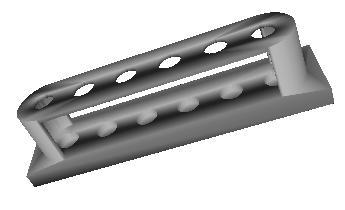
\includegraphics[scale=1]{Capt}
\caption{Figure 1}
\end{figure}
